% This file was created by matlab2tikz.
%
%The latest updates can be retrieved from
%  http://www.mathworks.com/matlabcentral/fileexchange/22022-matlab2tikz-matlab2tikz
%where you can also make suggestions and rate matlab2tikz.
%
\documentclass[]{standalone}
\usepackage{amsmath}
\usepackage{graphicx}
\usepackage[pdf]{pstricks}
\usepackage{pgfplots}
\pgfplotsset{compat=newest}
\usepgfplotslibrary{fillbetween}
%% the following commands are needed for some matlab2tikz features
\usetikzlibrary{plotmarks}
\usetikzlibrary{arrows.meta}
\usepgfplotslibrary{patchplots}
\usetikzlibrary{decorations.text}
\usetikzlibrary{shapes.multipart}


\newcommand{\logLogSlopeTriangle}[5]
{
	% #1. Relative offset in x direction.
	% #2. Width in x direction, so xA-xB.
	% #3. Relative offset in y direction.
	% #4. Slope d(y)/d(log10(x)).
	% #5. Plot options.
	
	\pgfplotsextra
	{
		\pgfkeysgetvalue{/pgfplots/xmin}{\xmin}
		\pgfkeysgetvalue{/pgfplots/xmax}{\xmax}
		\pgfkeysgetvalue{/pgfplots/ymin}{\ymin}
		\pgfkeysgetvalue{/pgfplots/ymax}{\ymax}
		
		% Calculate auxilliary quantities, in relative sense.
		\pgfmathsetmacro{\xArel}{#1}
		\pgfmathsetmacro{\yArel}{#3}
		\pgfmathsetmacro{\xBrel}{#1-#2}
		\pgfmathsetmacro{\yBrel}{\yArel}
		\pgfmathsetmacro{\xCrel}{\xArel}
		%\pgfmathsetmacro{\yCrel}{ln(\yC/exp(\ymin))/ln(exp(\ymax)/exp(\ymin))} % REPLACE THIS EXPRESSION WITH AN EXPRESSION INDEPENDENT OF \yC TO PREVENT THE 'DIMENSION TOO LARGE' ERROR.
		
		\pgfmathsetmacro{\lnxB}{\xmin*(1-(#1-#2))+\xmax*(#1-#2)} % in [xmin,xmax].
		\pgfmathsetmacro{\lnxA}{\xmin*(1-#1)+\xmax*#1} % in [xmin,xmax].
		\pgfmathsetmacro{\lnyA}{\ymin*(1-#3)+\ymax*#3} % in [ymin,ymax].
		\pgfmathsetmacro{\lnyC}{\lnyA+#4*(\lnxA-\lnxB)}
		\pgfmathsetmacro{\yCrel}{\lnyC-\ymin)/(\ymax-\ymin)} % THE IMPROVED EXPRESSION WITHOUT 'DIMENSION TOO LARGE' ERROR.
		
		% Define coordinates for \draw. MIND THE 'rel axis cs' as opposed to the 'axis cs'.
		\coordinate (A) at (rel axis cs:\xArel,\yArel);
		\coordinate (B) at (rel axis cs:\xBrel,\yBrel);
		\coordinate (C) at (rel axis cs:\xCrel,\yCrel);
		
		% Draw slope triangle.
		\draw[#5]   (A)-- node[pos=0.5,anchor=north] {1}
		(B)-- 
		(C)-- node[pos=0.5,anchor=west] {#4}
		cycle;
	}
}

\begin{document}
	
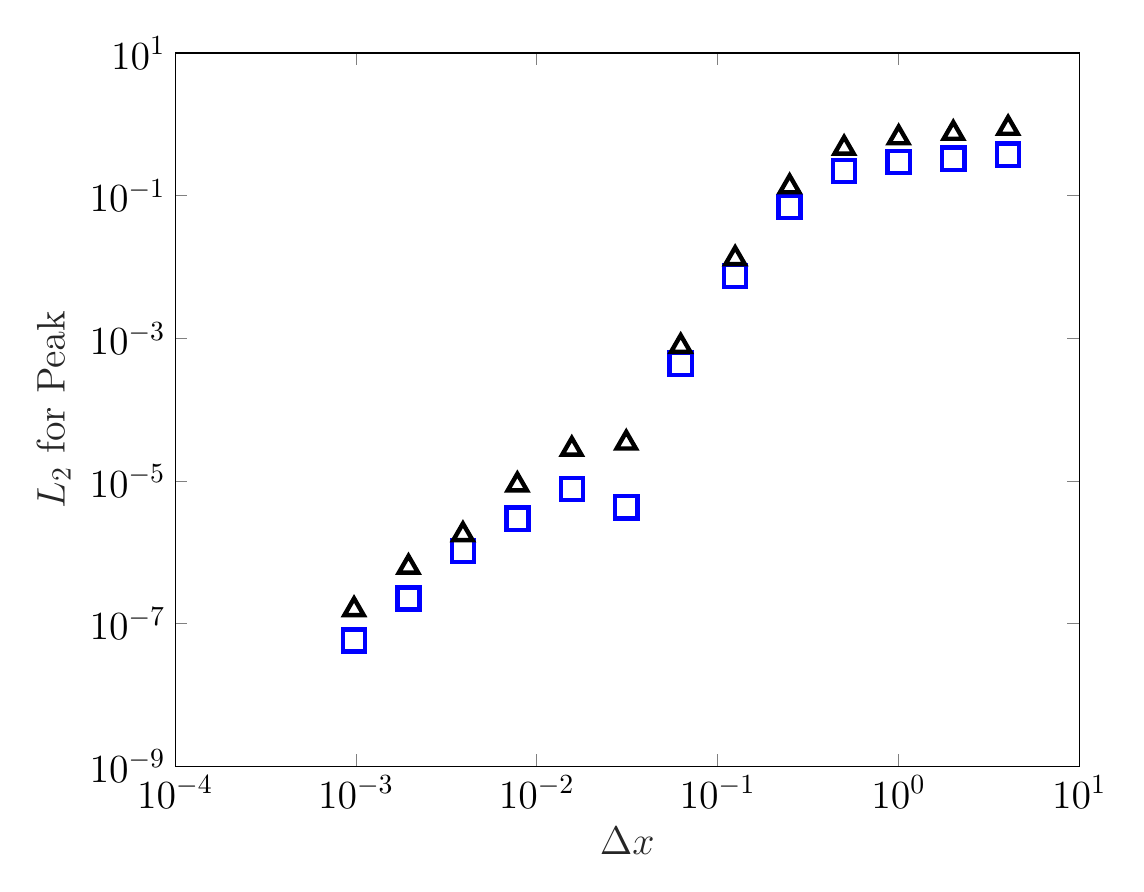
\begin{tikzpicture}
\tikzstyle{every node}=[font=\Large]
\begin{axis}[%
width=4.521in,
height=3.566in,
at={(0.758in,0.481in)},
every axis plot/.append style={ultra thick},
scale only axis,
xmode=log,
xmin=0.0001,
xmax=10,
xtick={0.0001,  0.001,   0.01,    0.1,      1,     10},
xminorticks=false,
xlabel style={font=\color{white!15!black}},
xlabel={\Large $\Delta x$},
ymode=log,
ymin=1e-09,
ymax=10,
ytick={1e-09, 1e-07, 1e-05, 0.001,   0.1,    10},
yminorticks=false,
ylabel style={font=\color{white!15!black}},
ylabel={\Large $L_2$ for Peak},
axis background/.style={fill=white}
]
 \logLogSlopeTriangle{0.45}{0.2}{0.09}{2}{black};

\addplot [color=blue, draw=none, mark=square, mark size=4pt, mark options={solid, blue}, forget plot]
  table[row sep=crcr]{%
4.04040404040404	0.374635819107519\\
2.01005025125628	0.330575957190649\\
1.00250626566416	0.295535139423467\\
0.500625782227785	0.222310290545868\\
0.250156347717323	0.0696546911351294\\
0.125039074710847	0.00752794654821404\\
0.0625097671511174	0.000440500513957322\\
0.0312524415969998	4.28287380384225e-06\\
0.0156256103754053	7.74963902109228e-06\\
0.00781265259087092	2.96103076228228e-06\\
0.00390628814734519	1.0494996245914e-06\\
0.00195313453678973	2.25578757111619e-07\\
0.000976564884191612	5.78813263985012e-08\\
};
\addplot [color=black, draw=none, mark=triangle, mark size=4pt, mark options={solid, black}, forget plot]
  table[row sep=crcr]{%
4.04040404040404	0.884133646659559\\
2.01005025125628	0.750902343165237\\
1.00250626566416	0.649994885480656\\
0.500625782227785	0.463780898088146\\
0.250156347717323	0.133659973869748\\
0.125039074710847	0.0131548809289435\\
0.0625097671511174	0.000774323155143161\\
0.0312524415969998	3.41065658067498e-05\\
0.0156256103754053	2.79244343909662e-05\\
0.00781265259087092	8.82186495229507e-06\\
0.00390628814734519	1.77009502620524e-06\\
0.00195313453678973	6.20579547916239e-07\\
0.000976564884191612	1.57661294328392e-07\\
};
\end{axis}
\end{tikzpicture}%
\end{document}